\documentclass[a4paper,12pt]{article}
\usepackage{amsmath,amsfonts,amsthm,amscd,amssymb,latexsym}%,eufrak}
%%%%%%%%%%%%%
\usepackage{caption}
\usepackage{subcaption}
\usepackage{enumerate,graphicx,psfrag}%,subfigure}%,jchangebar,oldgerm}
\usepackage[mathscr]{eucal}
\usepackage[usenames]{color}
\usepackage{url}
\usepackage[shortlabels]{enumitem}
\usepackage{comment}
%\usepackage[utf8]{inputenc}
\usepackage[T1]{fontenc}
%\usepackage{showkeys}
\usepackage{wrapfig}
\usepackage{lscape}
\usepackage{rotating}
%%%%%%%%%
\sloppy
%%%%%%%%%%%%%%%%%%%%%%%
\title{The subgroup membership problem in amalgamated products of 
finitely generated free groups
}
\author{Andrew J. Duncan, Elizaveta Frenkel}

\renewcommand{\a}{\alpha }
\renewcommand{\b}{\beta }
\newcommand{\G}{\Gamma }
\newcommand{\g}{\gamma }
\newcommand{\D}{\Delta }
\renewcommand{\d}{\delta }
%\def\vd{\vardelta}
\newcommand{\ep}{\epsilon }
\newcommand{\e}{\varepsilon }
\newcommand{\z}{\zeta }
%\eta
\renewcommand{\th}{\theta }
\newcommand{\T}{\Theta }
\renewcommand{\i}{\iota }
\renewcommand{\k}{\kappa }
\renewcommand{\l}{\lambda }
\renewcommand{\L}{\Lambda }
%\mu
%\nu
%\xi
%omicron
%\pi
\renewcommand{\r}{\rho }
\newcommand{\s}{\sigma }
\renewcommand{\S}{\Sigma }
\renewcommand{\t}{\tau }
\newcommand{\up}{\upsilon }
\newcommand{\U}{\Upsilon }
%\phi
\newcommand{\x}{\chi }
%\psi
\newcommand{\W}{\Omega }
\newcommand{\w}{\omega }
%%%%%%%%%%%%%%%%%%%%%%%%%%%%%%%
%%%%%%%%%%%%%%%%%%%%%%%%%%%%%
\newcommand{\pd}{\partial}
\newcommand{\wht}{\widehat}
%\newcommand{\cC}{{\mathcal C}}
%\newcommand{\cdim}{\texttt{cdim}}
\newcommand{\fC}{{\textswab C}}
\newenvironment{ef}{\noindent\color{blue} \bf EF: }{}
%
\newcommand{\cA}{{\cal{A}}}
\newcommand{\cD}{{\cal{D}}}
\newcommand{\cF}{{\cal{F}}}
\newcommand{\cH}{{\cal{H}}}
\newcommand{\cJ}{{\cal{J}}}
\newcommand{\cK}{{\cal{K}}}
\newcommand{\cP}{{\cal{P}}}
\newcommand{\cQ}{{\cal{Q}}}
\newcommand{\cR}{{\cal{R}}}
\newcommand{\cS}{{\cal{S}}}
\newcommand{\cV}{{\cal{V}}}
\newcommand{\cW}{{\cal{W}}}
%\newcommand{\GG}{\ensuremath{\mathbb{G}}}
\newcommand{\pp}{\mathbf{p}}
%%%%%%%%%%%%%%%%%%%%%%%%%%%%%%
\newcommand{\nul}{\emptyset }
\newcommand{\vim}{\nu\textrm{-im}}
%%%%%%%%%%%%%%%%%%%%%%%%%%%%%%
\newtheorem{theorem}{Theorem}[section]
\newtheorem{lemma}[theorem]{Lemma}
\newtheorem{corollary}[theorem]{Corollary}
\newtheorem{proposition}[theorem]{Proposition}
\newtheorem{axiom}[theorem]{Axiom}
\newtheorem{definition}[theorem]{Definition}
\newtheorem*{defn*}{Definition}
\newtheorem{conjecture}[theorem]{Conjecture}
%cvs -d :pserver:najd2@cvs.mas.ncl.ac.uk:/CVS/najd2
\newtheorem{exam}[theorem]{Example}
%\newtheorem{comment}[theorem]{Comment}
%
%
\newenvironment{example}{\begin{exam} \rm}{\end{exam}}
%
%
%
\newtheorem{remk}[theorem]{Remark}
\newenvironment{remark}{\begin{remk} \rm}{\end{remk}}
%
%%%%%%%%%%%%
\numberwithin{equation}{section}
\numberwithin{figure}{section}
%%%%%%%%%%%%%%%%%%%%
\newcommand{\Loop}{\operatorname{Loop}}
\newcommand{\Iso}{\operatorname{Isom}}
\newcommand{\Aut}{\operatorname{Aut}}
%%%%%%%%%%%%%%%%%%%
\renewcommand{\AA}{\ensuremath{\mathbb{A}}}
\newcommand{\ZZ}{\ensuremath{\mathbb{Z}}}
\newcommand{\QQ}{\ensuremath{\mathbb{Q}}}
\newcommand{\RR}{\ensuremath{\mathbb{R}}}
\newcommand{\NN}{\ensuremath{\mathbb{N}}}
\newcommand{\CC}{\ensuremath{\mathbb{C}}}
\newcommand{\FF}{\ensuremath{\mathbb{F}}}
%\renewcommand{\ker}{\verb"Ker"}
\newcommand{\cC}{\mathcal{C}}
\renewcommand{\cF}{\mathcal{F}}
\newcommand{\cO}{\mathcal{O}}
\renewcommand{\cS}{\mathcal{S}}
\newcommand{\la}{\langle}
\newcommand{\ra}{\rangle}
%\newcommand{\BA}{\ensuremath{\mathbb{A}}}
%%%%%%%%%%%%%%%%%%%%%%%%%%%%%%%%%%%%%%
\newcommand{\maps}{\rightarrow}
\newcommand{\ov}[1]{\overline{#1}}
\newcommand{\bs}{\backslash}
%%%%%%%%%%%%%%%%%%%%%%%%%%%%%%%
\newcommand{\be}{\begin{enumerate}}
\newcommand{\ee}{\end{enumerate}}
\newcommand{\bd}{\begin{description}}
\newcommand{\ed}{\end{description}}
\newcommand{\biz}{\begin{itemize}}
\newcommand{\eiz}{\end{itemize}}
%%%%%%%%%%%%%%%%%%%%%%%%%%%%%%%%%%%
%
\newenvironment{ajd1}{\noindent\color{red} AJD }{}
\newcommand{\ajd}[1]{\begin{ajd1} #1 \end{ajd1}}
%
%\includecomment{comp}% to see environment comp
\excludecomment{comp}% to hide environment comp
%
\begin{document}
$F_1=F( x_1,x_2)$, $F_2=F(y_1, y_2)$, $H_1=\la x_2x_1^{-1}, x_2^3, x_2x_1x_2,
x_1^{-1}x_2\ra$, $H_2$ is the same with $y_1$ instead of $x_1$ and $y_2$ instead
of $x_2$. $\phi_1$ maps $z_1$ to $  x_2x_1^{-1}$, $z_2$ to $x_2^3$, $z_3$ to 
 $x_2x_1x_2$ and $z_4$ to $x_1^{-1}x_2$. $\phi_2$ does the same but 
with the $'$ added. $H_k$ is normal in $F_k$.
The Stallings folding for $H_1$ is shown in the figure.
\begin{figure}
\begin{center}
\psfrag{a1}{$x_1|z_1^{-1}$}
\psfrag{a2}{$x_1|z_3$}
\psfrag{a3}{$x_1|z_4^{-1}$}
\psfrag{b1}{$x_2|1$}
\psfrag{b2}{$x_2|z_2$}
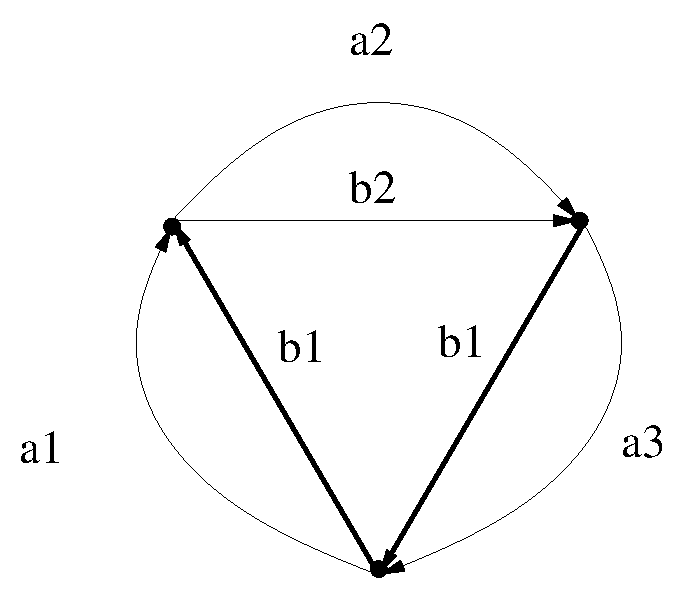
\includegraphics[scale=0.6]{ce.eps}
\end{center}
\end{figure}

$K=\la y_1x_1,x_1^{-1}x_2\ra$. 


I constructed our generalised 
folding for $K$: of course I may have made mistakes, but it
looks like it does not accept what it should. 

In particular, as it's normal, we have
in $H_1$, elements of the form
\[
x_1^n (x_1^{-1}x_2)x_1^{-n} = x_1^{n-1}x_2x_1^{-n},\]
for $n\ge 1$.
To put these in normal form it helps to calculate 
$x_1^3=
x_1x_2^{-1}\cdot x_2x_1x_2\cdot x_2^{-1}x_1=z_1^{-1}z_3z_4^{-1}$.
(Although I wouldn't do so: it's easier to read the normal form off the Stallings folding 
for $H_k$.)
Let's consider the case $n-1\ge 0$ (the other case won't be much different).
Then $n-1=3q+r$, where $q\ge 0$ and $0\le r<3$. I seem to have to 
do this case by case, so here goes. When $r=0$
\[x_1^{n-1}x_2x_1^{-n}=x_1^{3q}x_2x_1^{-1}x_1^{-3q}=(z_1^{-1}z_3z_4^{-1})^q z_1 (z_1^{-1}z_3z_4^{-1})^{-q}.\]
 When $r=1$ 
\[
x_1^{n-1}x_2x_1^{-n}=x_1^{3q}x_1x_2x_1^{-2}x_1^{-3q}=(z_1^{-1}z_3z_4^{-1})^q z_1^{-1}z_2 z_3^{-1}z_1
(z_1^{-1}z_3z_4^{-1})^{-q}.
\]
When $r=2$
\begin{align*}
x_1^{n-1}x_2x_1^{-n}&=x_1^{3q}x_1^2x_2x_1^{-3(q+1)}=(z_1^{-1}z_3z_4^{-1})^q z_1^{-1}z_3 
(z_1^{-1}z_3z_4^{-1})^{-(q+1)}\\&=(z_1^{-1}z_3z_4^{-1})^q z_1^{-1}z_3z_4z_3^{-1}z_1 
(z_1^{-1}z_3z_4^{-1})^{-q}.
\end{align*}
All these are reduced as written. 
If we apply $\phi_2$ to the right hand side of each of these three equations we see that 
the left hand side, with $'$ added, belongs to $H_2$, in each case. 
In particular, in $H_1$ we have 
\begin{align*}
x_1x_2x_1^{-2}&=z_1^{-1}z_2z_3^{-1}z_1\\
x_1^2x_2x_1^{-3}&= z_1^{-1}z_3z_4z_3^{-1}z_1\\
x_1^3x_2x_1^{-4}&=  z_1^{-1}z_3z_4^{-1}z_1z_4z_3^{-1}z_1\\
x_1^4x_2x_1^{-5}&= z_1^{-1}z_3z_4^{-1}z_1^{-1}z_2z_3^{-1}z_1z_4z_3^{-1}z_1
\end{align*}

Now, in $K$ we have
\[
y_1x_1 (x_1^{-1}x_2) x_1^{-1}y_1^{-1}= y_1(x_2x_1^{-1})y_1^{-1}= y_1y_2y_1^{-1}y_1^{-1}=y_1y_2y_1^{-2},
\]
which is in $K\cap H_2$, by the above. Thus, in $G$ we have 
$y_1y_2y_1^{-2}=x_1x_2x_1^{-2}\in K\cap H_1$. Now assume that for some even $n>0$ we have
$x_1^{n-1}x_2x_1^{-n}\in K\cap H_1$. Then   
\begin{align*}
y_1x_1(x_1^{n-1}x_2x_1^{-n})x_1^{-1}y_1^{-1}&=y_1(x_1^nx_2x_1^{-(n+1)})y_1^{-1}\\
&=y_1(y_1^ny_2y_1^{-(n+1)})y_1^{-1}\\
&=y_1^{n+1}y_2y_1^{-(n+2)}\in K\cap H_2,
\end{align*}
and applying $\phi_1\phi_2^{-1}$ we see that $x_1^{n+1}x_2x_1^{-(n+2)}\in K\cap H_1$. 
Thus $x_1^{n-1}x_2x_1^{-n}\in K\cap H_1$, for all even $n\ge 0$. 

My generalised folding doesn't even accept the normal form of the first non-trivial
elemenent of this list: $z_1^{-1}z_2z_3^{-1}z_1$.

I think the problem may be that the normal form is not unique
for elements of $K$. For example
$y_1x_1 = z_1^{-1} y_2 z_1^{-1}x_2$, which is it's normal form, but
also 
\[y_1x_1=y_1y_2^{-1}y_2x_1x_2^{-1}x_2=y_1y_2^{-1}y_2y_1y_2^{-1}x_2=y_1y_1y_2^{-1}x_2=
z_1^{-1}z_3z_2^{-1}y_2x_2,\]
which is in normal form. 

I think you were telling me you know how to get round this. I'll have a
look at the ``Tale of Two Authors'', and see if I understand. 

\ajd{There was a mistake: at the end of the proof of Theorem 3.2 in our paper.
Here the subgroups are forced to be malnormal, which makes the theorem better
again.}
\begin{theorem}\label{thm:dcnf} Let $D_1$ and $D_2$ be sets of  double coset representatives for
$H_1\le F_1$ and $H_2\le F_2$, respectively. \ajd{Assume that
$H_i$ is malnormal in $F_i$, $i=1,2$.}  
Then every element of $G$ is represented by a unique element of
$\FF(X_1\cup X_2\cup Z)$ in double coset normal form, with respect
to $D_1\cup D_2$.
\end{theorem}
\begin{proof}
To see that every $g\in G$ can be written in dc-normal form, first
write $g$ in reduced form. If the reduced form of $g$ is the empty
word then this is also the dc-normal form; with $k=0$ and $h_0=1$. 
Otherwise we have $g=f_1\cdots f_t$, where $f_i$ is in $F_{j_i}$, for
$j_i\in \{1,2\}$. In this case, let $a_is_ib_i$
be the double coset representative of $f_i$, where 
$a_i,b_i\in H_{j_i}$ and $s_i\in D_{j_i}$. For $i=1,\ldots ,t$,
 let $z^{\prime}_i=\phi_j^{-1}(a_i)$ and
$z^{\prime\prime}_i=\phi_j^{-1}(b_i)$. For $i=1,\ldots ,t-1$, let 
$z_i$ be the free reduction of $z^{\prime}_iz^{\prime\prime}_{i+1}$, 
and let $z_0=z^{\prime}_1$ and $z_t=
z^{\prime\prime}_t$. 
 If $t=1$ and $f_1\in H_{j_1}$ then $a_1=f_1$, $s_1=1$, $b_1=1$ and 
the dc-normal form of $g$ is $z_0$. Otherwise, for all $i\ge 1$, we 
have $f_i\notin H_1\cup H_2$, so $s_i\neq 1$ and 
\[z_0s_1z_1\cdots z_{t-1}s_tz_t\]
is a dc-normal form for $g$.

Now suppose that $w$ and $w^\prime$ are words in dc-normal form and that
$w=_G w^\prime$. We show by induction on $k$ that $w=w'$. 
Let $w=h_{0}p_1h_{1}p_2 \cdots h_{k-1}p_kh_{{k}}$,
and $w^\prime =h_{0}^\prime p_1^\prime h_{1}^\prime  p_2^\prime
\cdots h_{k-1}^\prime p_k^\prime h_{{k^\prime}}^\prime$, where
$h_i, h_i^\prime\in \FF(Z)$ and $p_i,p_i^\prime\in S_1\cup S_2$.
If $k=0$ let $f_1=\phi_1(h_0)$ and, if $k>0$, 
let $f_1=\phi_{j_1}(h_0)p_1\phi_{j_1}(h_1)$, where $p_1\in F_{j_1}$. 
 In addition, if $k>0$,  
 for fixed $i\ge 2$, assuming that $p_i\in F_{j_i}$, 
let $f_i=p_i\phi_{j_i}(h_i)$.
 Then $f_1\cdots f_k$, is
a reduced form for the element $w\in G$. Similarly, we obtain a reduced
form $f_1^\prime \cdots f_{k^\prime}^\prime$, for $w^\prime=_G w$,\ajd{ 
with
$f_i'=p'_i\phi_{j'_i}(h'_i)$, $p_i'\in H_{j'_i}$}. 

If $k=0$ then we have $w=_G f_1=\phi_1(h_0)\in H_{1}$, and since all 
reduced forms representing an element have the same length, $k'=0$ or $1$. 
Moreover, as $f'_1=_G w\in H_1$ we have 
 $k^\prime =0$ and $w^\prime=_G f_1^\prime=\phi_1(h_0^\prime)\in H_1$.
As $H_1$ embeds in $G$ this implies that $\phi_1(h_0)=\phi_1(h'_0)$, so
$w=h_0=h'_0=w'$. Thus the result
holds when $k=0$ and we may assume inductively that $k>0$ and the result holds
for elements represented by normal forms of length less than $k$.

Comparing the lengths of reduced forms, we have $k=k^\prime$.
Moreover, $1=_G w^\prime w^{-1}= f_1^\prime \cdots f_{k}^\prime
f_k^{-1}\cdots f_1^{-1}$, so by \cite[Chapter IV, Theorem 2.6]{LS}, 
we have \ajd{$ f_{k}^\prime f_k^{-1}\in H_{1}\cup H_2$.
Assume first that $k>1$. 
In this case, 
\[ f_{k}^\prime f_k^{-1}= p'_k\phi_{j_k'}(h'_k)\phi_{j_k}(h_k^{-1})p_k^{-1}\in H_1\cup H_2.\] 
 Hence, $j_k=j'_k$ and 
$f_{k}^\prime f_k^{-1}=
p'_k\phi_{j_k}(h'_k h_k^{-1})p_k^{-1}\in H_{j_k}$; 
so $p_k'\in H_{j_k}p_k\phi_{j_k}(h_k (h'_k)^{-1})$ and therefore, as 
$p_k, p'_k$ are  double coset representatives,  
$p_k'=p_k$. 
Thus $p_k\phi_{j_k}(h'_k h_k^{-1})p_k^{-1}\in H_{j_k}$, and as 
$H_{j_k}$ is malnormal in $F_{j_k}$, this implies that
$\phi_{j_k}(h'_k h_k^{-1})$ and so $h_k=h'_k$.\\
This didn't happen before because $H_{j_k}$ was not 
necessarily malnormal.\\
Now suppose that $k=1$. Then 
\[
f_{1}^\prime f_1^{-1}=\phi_{j_1'}(h'_0) p'_1\phi_{j_1'}(h'_1)
\phi_{j_1}(h_1^{-1})p_1^{-1}\phi_{j_1}(h_0^{-1})\in H_1\cup H_2.
\] 
Again, $j_1=j'_1$ and so we
 have $p'_1\phi_{j_1'}(h'_1)\phi_{j_1}(h_1^{-1})p_1^{-1}
\in H_{j_1}$, 
and as in the case $k>1$ this implies that $p_1=p'_1$ and 
$h_1=h'_1$. It now follows that also $h_0=h_0'$. 
 
Hence, in all cases, $f_k=f'_k$. 
Therefore the reduced forms 
$f_1\cdots f_{k-1}$ and 
$f_1^\prime \cdots f_{k-1}^\prime$ both represent the same 
element of $G$. From the inductive assumption we have 
$h_0=h_0'$,  $h_i=h'_i$ and $p_i=p'_i$, for $i=1,\ldots, k-1$. 
Thus }
   $w=w^\prime$, as required.
\end{proof}

The problem is with length $k=1$ when we are comparing 
$f_1=\phi_{j_i}(h_0)p_1\phi_{j_i}(h_1)$ with the corresponding $f'_1$. 
To see what might (and does) go wrong, consider the above example; cut down
a bit. 
Here we have two normal forms for the element
 $y_2y_1y_2^{-2}x_2=_Gx_2y_1y_2^{-1}$, namely
\[z_3z_2^{-1}x_2=_G x_2z_1^{-1}.\]
In this case $h_0=z_3z_2^{-1}$, $p_1=x_2$, $h_1=1$, $h'_0=1$, $p'_1=x_2$ and 
$h'_1=z_1^{-1}$. 

To see how this equality arises:
\[x_2z_1^{-1}x_2^{-1}=x_2(x_1x_2^{-1})x_2^{-1}=(x_2x_1x_2)(x_2^{-3})=z_3z_2^{-1}.\]
There is no problem with $k>1$, because then the comparison is between
$f_k=p_k\phi_{j_i}(h_k)$ and $f'_k$, of the analogous form. It is the 
difficulty of conjugating one element of $H_k$ to another that causes
the problem, and this only bothers us when $k=1$. 

I still hope our double coset representatives are unique: I'm pretty sure
they are, but haven't checked the proofs. The element above 
$z_3z_2^{-1}x_2=_G x_2z_1^{-1}$, if regarded as an element of $F_1$, that is
as $(x_2x_1x_2)(x_2^{-3})x_2=x_2x_1x_2^{-1}$, has uniqe dc representative, namely $x_2$, and 
would be written as $x_2(x_1x_2^{-1})\in H_1x_2H_1$.
(All reps are of type 2 as the subgroup is normal.)

The same sort of problem seems to arise with our original example, in the paper.
In that case, suppose we take a subgroup $K$ generated by a set including the 
element $y_2x_1$. In this $G$ we have
$y_2^2=x_1^3$, so $y_2x_1=y_2(y_2^2x_1^{-3})x_1=y_2^3x_1^{-2}$. The dc normal 
form of $y_2x_1$ is $z_1y_2^{-1}x_1$ while the dc normal form of $y_2^3x_1^{-2}$
 is $z_1^2y_2^{-1}z_1^{-1}x_1$.

These two normal forms are equal in $G$ if and only if $z_1y_2^{-1}= z_1^2y_2^{-1}z_1^{-1}$
if and only if $y_2=z_1y_2z_1^{-1}$, if and only if $y_2$ is pn with respect to $H_2$. As this is the case, there are infinitely many normal forms
for the element $y_2x_1$: namely $z_1^{n+1}y_2^{-1}z_1^{-n}x_1$. 
\end{document}